\section {MAINTENANCE}

\textit{Maintenance} tab inform user about required inspection of machine or needed changed oil of fore pump. Shows information about how many hours fore pump worked from last oil changed and gives us information how many hours machine was  operating and how many processes was executed.\\

User can schedule when will be next maintenance by set exact date or set interval of time. When was time to maintenance, user will be informed by message on main window of application.\\

From this tab user can diagnosis chamber in terms of leak air. This purpose we should set threshold of pressure for pumping down of chamber and time of measurement of leak. Procedure of \textit{Leak Test} at first pumped down chamber to settings of threshold pressure and switched off fore pump. By time of measurement of leak, air leak will be measuring. When time passes, leakage rate will be calculated and showed to user.

	\begin{figure}[!h] 
	\centering 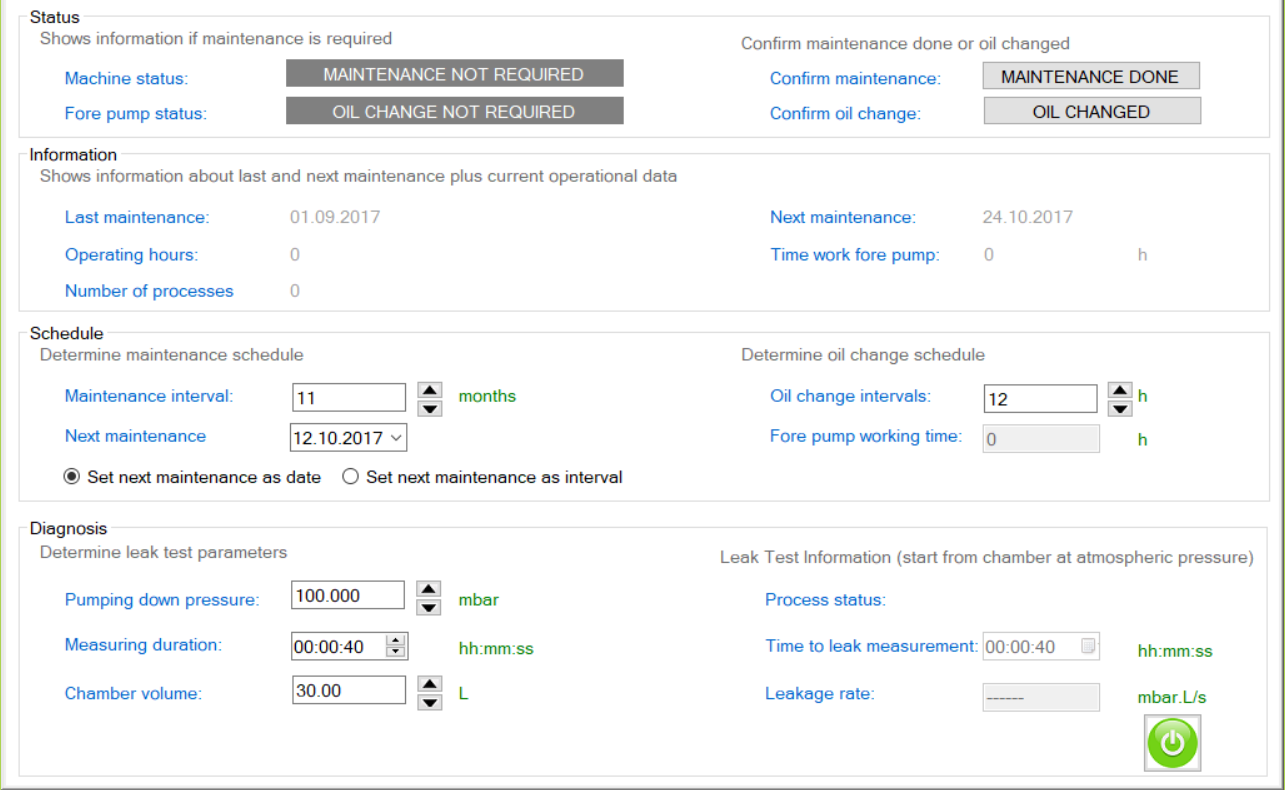
\includegraphics[width=0.7\textwidth]{Graphic/Maintenace/MaintenaceWindow.png}	
	\caption{Maintenace window}
	\label{maintenace_window}
	\end{figure}
	\FloatBarrier
